% begin module natural-exponential-ex7
\begin{frame}
\begin{example}[Example 6, p. 277]
\begin{columns}[c]
\column{.4\textwidth}
\ \only<handout:0| -5>{%
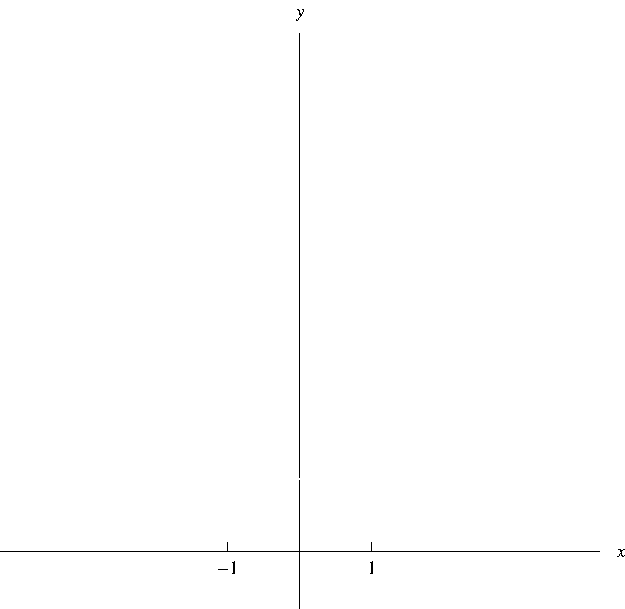
\includegraphics[height=5cm]{exponential-functions/pictures/07-02-ex7a.pdf}%
}%
\only<handout:0| 6-7>{%
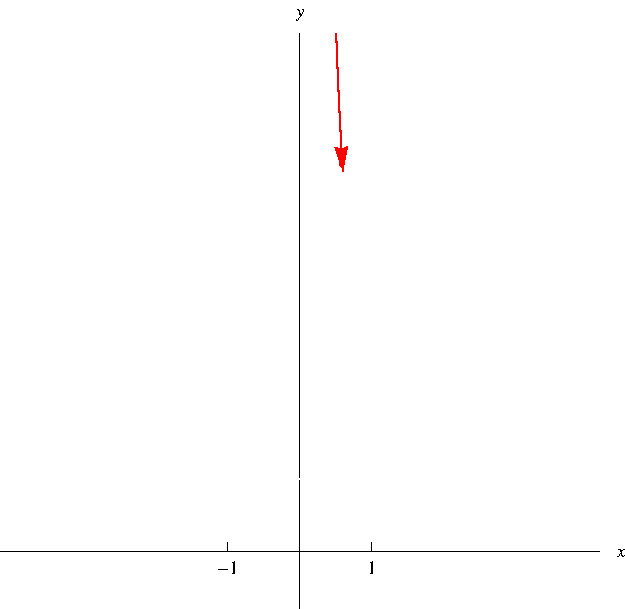
\includegraphics[height=5cm]{exponential-functions/pictures/07-02-ex7b.pdf}%
}%
\only<handout:0| 8-9>{%
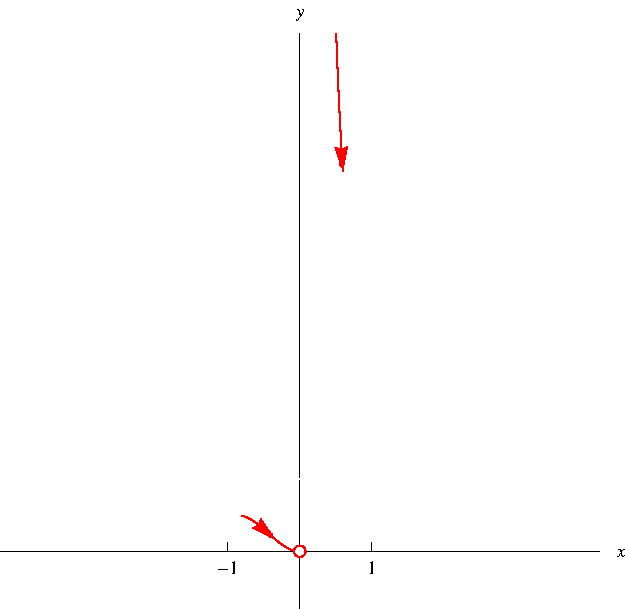
\includegraphics[height=5cm]{exponential-functions/pictures/07-02-ex7c.pdf}%
}%
\only<handout:0| 10-20>{%
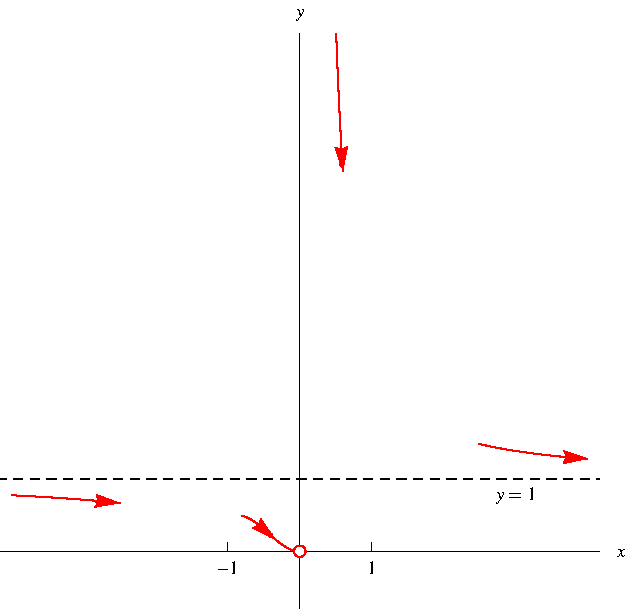
\includegraphics[height=5cm]{exponential-functions/pictures/07-02-ex7e.pdf}%
}%
\only<21->{%
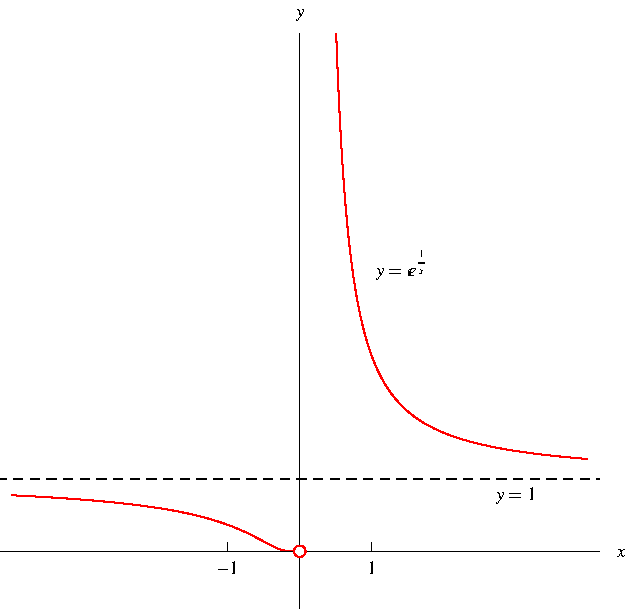
\includegraphics[height=5cm]{exponential-functions/pictures/07-02-ex7f.pdf}%
}%
\column{.6\textwidth}
\qquad Draw the graph of $f(x) = e^{1/x}$.
\begin{itemize}
\item<2->  $f(x)$ is always positive.
\item<3->  Domain: everything but 0.
\item<4->  Check for vertical asymptote at 0.  
\item<4->  $\displaystyle t = 1/x: \lim_{x\rightarrow 0^+} e^{1/x} \uncover<5->{ = \lim_{t\rightarrow\infty}e^t} \uncover<6->{ = \infty .}$
\item<4->  $\displaystyle t = 1/x: \lim_{x\rightarrow 0^-} e^{1/x} \uncover<7->{ = \lim_{t\rightarrow -\infty}e^t} \uncover<8->{ = 0.}$
\item<9->  As $x\rightarrow \pm \infty$, $1/x \rightarrow 0$.
\item<10->  Therefore $\lim_{x\rightarrow \pm \infty} e^{1/x} = 1$
\item<10->  $y = 1$ is a horizontal asymptote.
\end{itemize}
\end{columns}
\abovedisplayskip=0pt
\belowdisplayskip=0pt
\abovedisplayshortskip=0pt
\belowdisplayshortskip=0pt
\begin{align*}
\uncover<11->{f'(x) } & \uncover<11->{ = e^{1/x}\alert<handout:0| 12-13>{(1/x)'}} \uncover<12->{ = e^{1/x}\alert<handout:0| 12-13>{( \uncover<13->{-x^{-2}} )}} \uncover<14->{ = \alert<handout:0| 17-18>{-e^{1/x}/x^2}.} \\
\uncover<15->{f''(x)} & \uncover<15->{ = -\frac{(x^2) ( - e^{1/x}/x^2) - (e^{1/x})(2x)}{x^4}} \uncover<16->{ = \alert<handout:0| 19-20>{\frac{e^{1/x}(1+2x)}{x^4}}.}
\end{align*}
\alert<handout:0| 18>{\uncover<18->{Always decreasing.}}  \alert<handout:0| 20>{\uncover<20->{Inflection point: $(-1/2, e^{-2})$.}} 
\end{example}
\end{frame}
% end module natural-exponential-ex7
